%\VignetteIndexEntry{The Pviz users guide}
%\VignetteDepends{Pviz}
%\VignetteKeywords{Visualization}
%\VignettePackage{Pviz}
\documentclass[11pt]{article}
\usepackage{Sweave}
\usepackage[hmargin=2cm, vmargin=3cm]{geometry}


\author{Renan Sauteraud\footnote{rsautera@fhcrc.org}}

\begin{document}
\title{The Pviz User Guide}
\maketitle

\tableofcontents

%\newpage

\section{Introduction}
\texttt{Pviz} is an R package inspired by and depending on \texttt{Gviz}. It
introduces new types of track and extends the existing ones in order to deal
with amino-acid based data.

This package keeps most of the mechanics of \texttt{Gviz}, notably the use of
\texttt{DisplayParameters} and the same plotting function: \texttt{plotTracks}.
Therefore, the user is invited to refer to \texttt{Gviz} help pages and vignette
for more information and examples.

As with any R package, it should first be loaded in the session
\begin{Schunk}
\begin{Sinput}
> library(Pviz)
\end{Sinput}
\end{Schunk}



\section{Gviz tracks}
\texttt{Pviz} extends and uses the most common classes of \texttt{Gviz} to make
them easier to use with amino acid data. We removed the requirement for a genome
and a chromosome when creating these tracks. Moreover, they support the
functions defined in Pviz.

\subsection{ATrack}
\texttt{ATrack} extends Gviz's \texttt{AnnotationTrack} and behave the same way.
However, it does not require to specify a chromosome and a genome. Please refer
to \texttt{Gviz} documentation for more details about \texttt{AnnotationTrack}
and the available \texttt{DisplayParameters}.
\begin{Schunk}
\begin{Sinput}
> at <- ATrack(start = c(250, 480), end = c(320, 520), name = "Annotations")
> plotTracks(at, from = 1, to = 600)
\end{Sinput}
\end{Schunk}

\includegraphics{Pviz-ATrack-example}

\subsection{DTrack}
Naturally \texttt{DTrack} extends Givz's \texttt{DataTrack}. Here again, please
refer to \texttt{Gviz} documentation for details on how to use
\texttt{DataTrack}.

Some example data are available in this package. Expression frequency for
peptide in hxb2 envelope.
\begin{Schunk}
\begin{Sinput}
> data(PvizVignette)
> dt <- DTrack(data = freqEx, start = posEx, width = 15, name = "Freq")
> plotTracks(dt, from = 1, to = 850, type = "l")
\end{Sinput}
\end{Schunk}
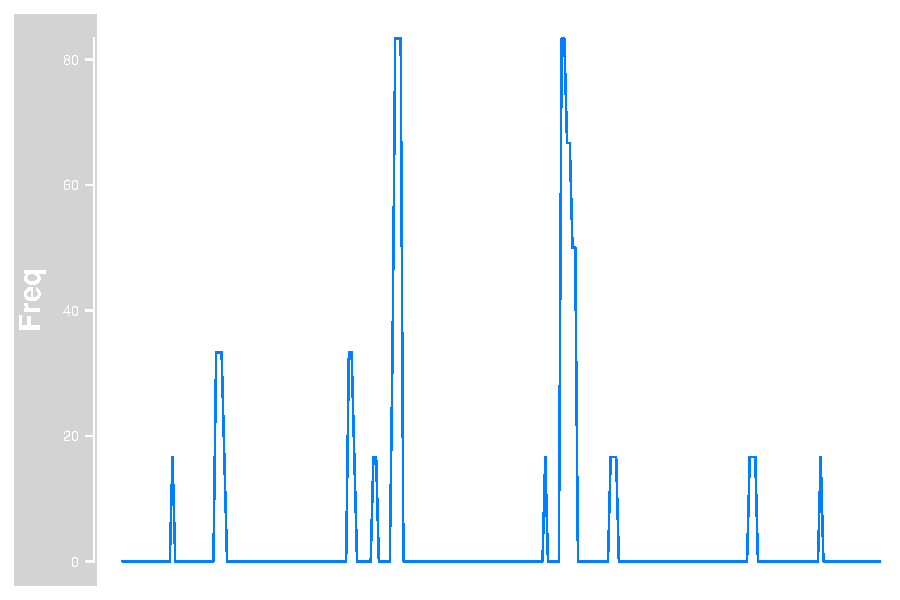
\includegraphics{Pviz-DTrack-example}


\section{Pviz new track types}
\texttt{Pviz} introduce some new track types to deal with amino-acid based data.
The new tracks look can be modified using the \texttt{DisplayParameters} and
will most of the time offer the same options as the ones available for
\texttt{Gviz} tracks.

\subsection{ProteinAxisTrack}
This track acts as a replacement for the \texttt{GenomeAxisTrack}. I comes
with the same coloration, transparency and other customization options but loses
the DNA representation for a simple segment.

\begin{Schunk}
\begin{Sinput}
> pat <- ProteinAxisTrack()
> plotTracks(pat, from = 1, to = 850)
\end{Sinput}
\end{Schunk}
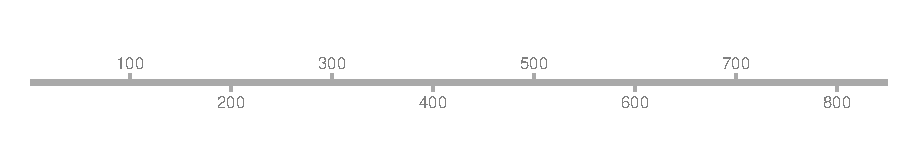
\includegraphics{Pviz-ProteinAxisTrack-basic}

Just like in \texttt{GenomeAxisTrack}, it is possible to use littleTicks to get
a more precise scale. Moreover, because \texttt{Pviz}, has been made to deal
with peptides and protein, the option addNc can display indicators for N-term
and C-term ends on the axis.

\begin{Schunk}
\begin{Sinput}
> pat <- ProteinAxisTrack(addNC = TRUE, littleTicks = TRUE)
> plotTracks(pat, from = 1, to = 850)
\end{Sinput}
\end{Schunk}
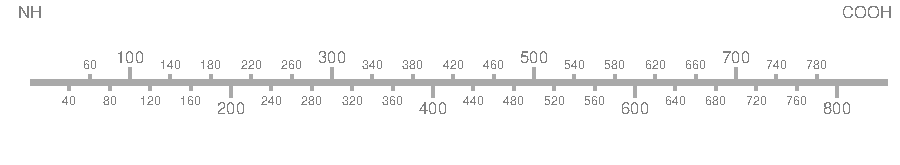
\includegraphics{Pviz-ProteinAxisTrack-options}

\subsection{SequenceTrack}
This new track simply displays a selected sequence. It can takes both
\texttt{AAstring} or regular \texttt{string} and thus, can be used for both
AA and DNA sequences.

Note that the first amino acid of the sequence should correspond to the first
position of any other element you choose to display at the same time.

The previously loaded dataset also contains an \texttt{AAstring} object for the
sequence of the envelope of hxb2.
\begin{Schunk}
\begin{Sinput}
> seqEx
\end{Sinput}
\begin{Soutput}
  857-letter "AAString" instance
seq: MRVKEKYQHLWRWGWRWGTMLLGMLMICSATEKLWV...VAEGTDRVIEVVQGACRAIRHIPRRIRQGLERILL*
\end{Soutput}
\begin{Sinput}
> st <- SequenceTrack(sequence = seqEx, name = "env")
> plotTracks(trackList = c(pat, st), from = 1, to = 50)
\end{Sinput}
\end{Schunk}
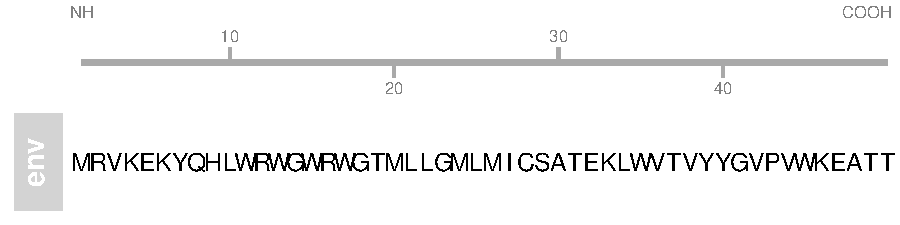
\includegraphics{Pviz-SequenceTrack-basic}

Note that if the plotting ranges becomes too wide, the letters will stack and it
may lead to an unreadable output. The default parameters usually allows to plot
up to 100-150 characters depending on your graphic window. The user can modify
the character size via the DisplayParameters system when creating the track
with the cex argument.
Here is an example of bad plotting.
\begin{Schunk}
\begin{Sinput}
> plotTracks(trackList = c(pat, st), cex = 0.5)
\end{Sinput}
\end{Schunk}
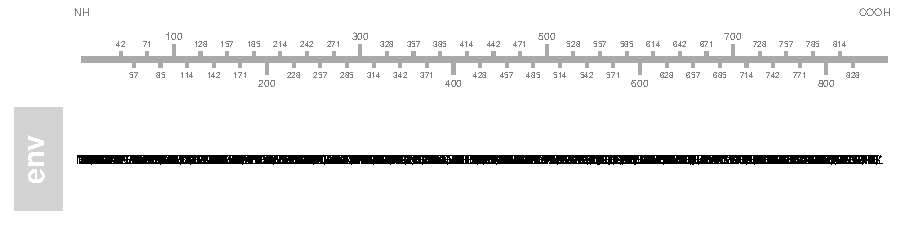
\includegraphics{Pviz-SequenceTrack-unreadable}

Althought the character expansion has been set to less than 1. The ranges are
still too wide for a correct display.

\subsection{ProbeTrack}
This track is designed to display peptide microarray data. It draws each peptide
relative to its position in the sequence and enclose them in rectangles colored
depending on their intensity.
To create this track, the sequence of the peptides, their intensity or
frequency and their starting position have to be passed as arguments.
\begin{Schunk}
\begin{Sinput}
> pt <- ProbeTrack(pepEx, freqEx, posEx)
> plotTracks(pt, from = 460, to = 530)
\end{Sinput}
\end{Schunk}
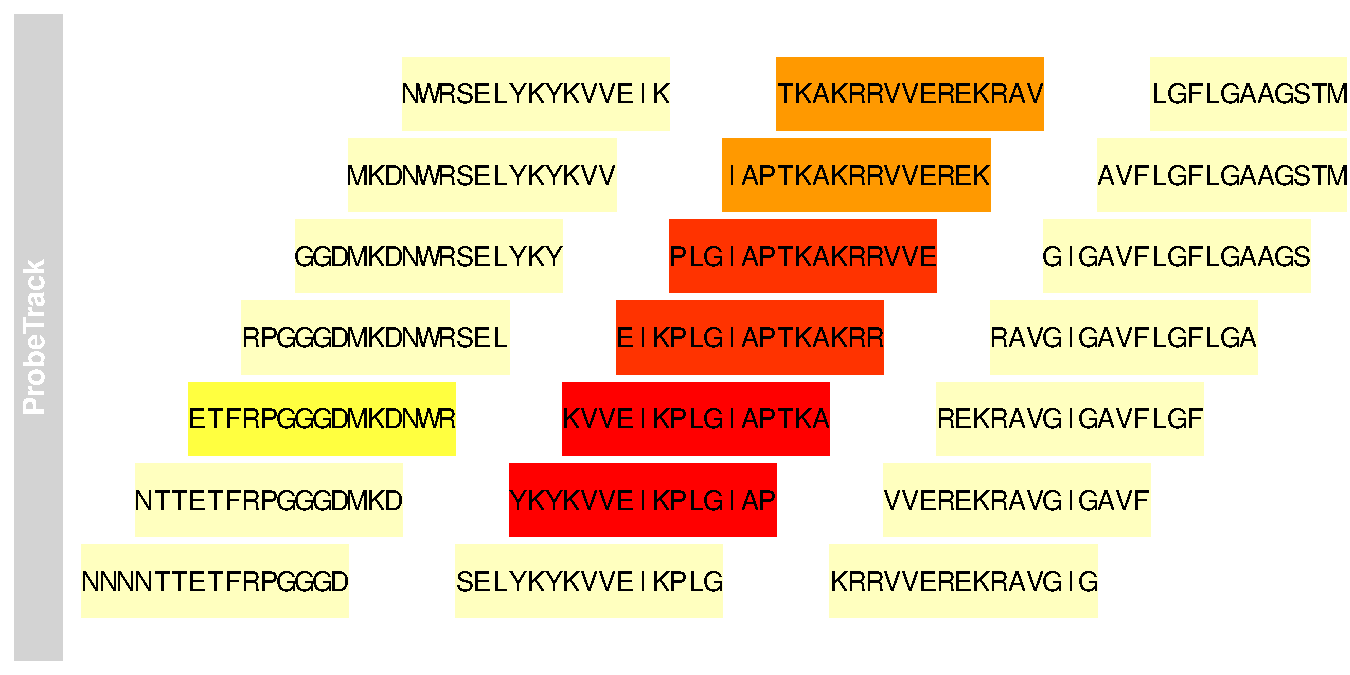
\includegraphics{Pviz-ProbeTrack-basic}

Unlike in \texttt{SequenceTrack}, the size of the characters in each peptide
sequence depends on the plotting ranges (the user can still choose to change the
size manually) and if the ranges become too wide, the characters will appear as
dots or completely disappear instead of stacking on top of each other.
While it loses the sequence information, it might be relevant to locate regions
where peptides have high intensity/frequency.
\begin{Schunk}
\begin{Sinput}
> plotTracks(pt)
\end{Sinput}
\end{Schunk}
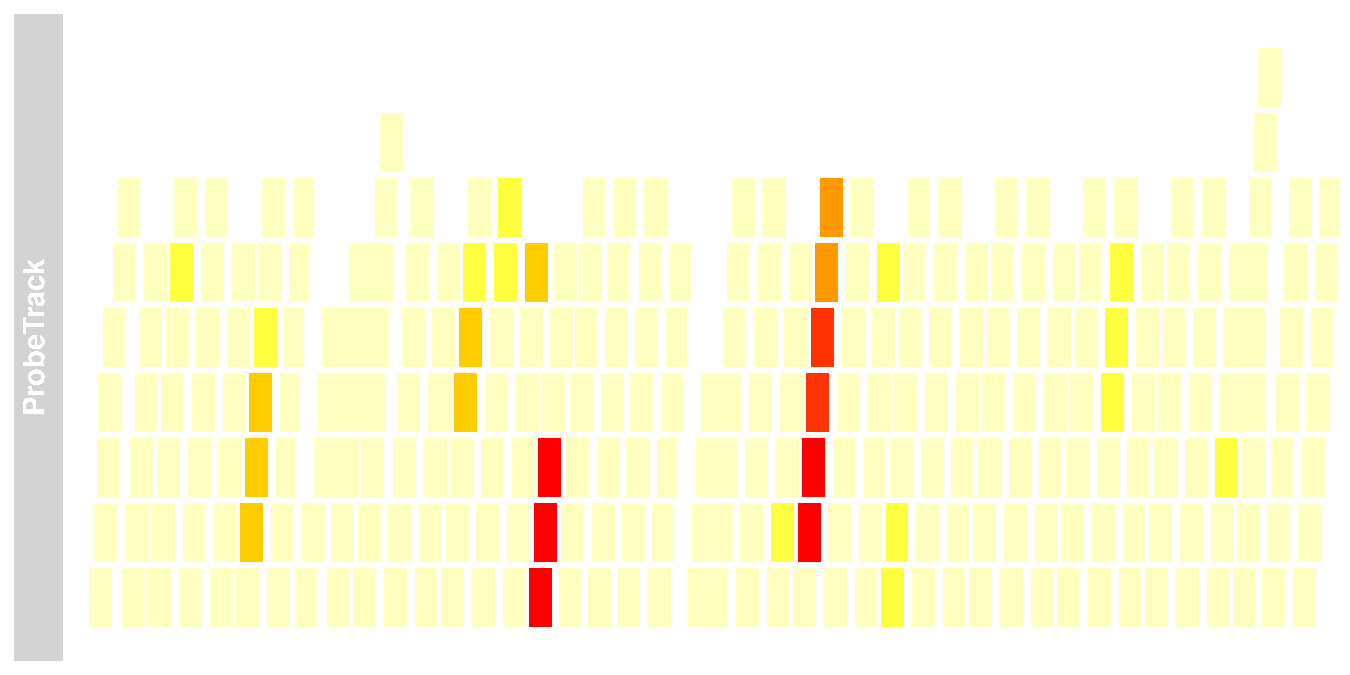
\includegraphics{Pviz-ProbeTrack-wide-ranges}

For a more explicit display, a legend has been implemented for this track and
can be called during track creation or in the plotting function. The legend
displays the scale of intensities.
\begin{Schunk}
\begin{Sinput}
> plotTracks(pt, from = 460, to = 530, legend = TRUE)
\end{Sinput}
\end{Schunk}
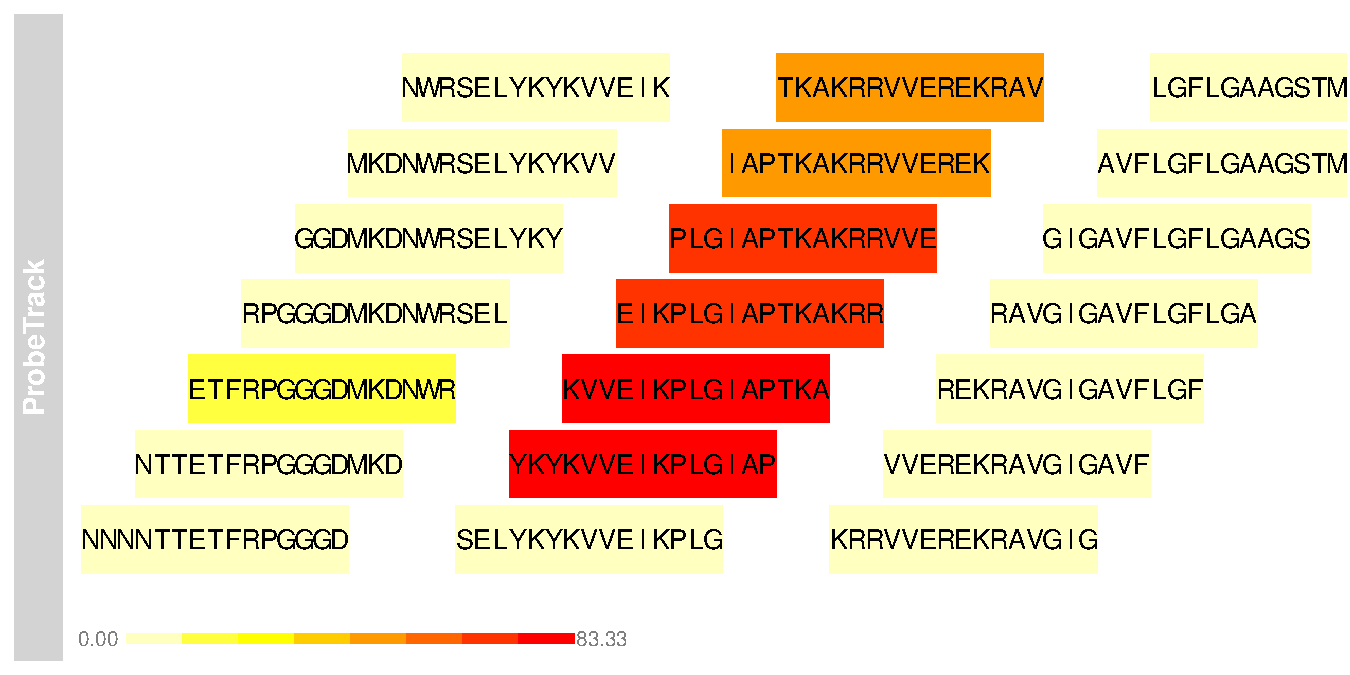
\includegraphics{Pviz-ProbeTrack-legend}





\section{Example of plot}
Naturally, the interest of \texttt{Pviz}, just like its parent \texttt{Gviz}
is the display of multiple tracks at once.
Here is an example of what \texttt{Pviz} can render, using the tracks previously
created.
\begin{Schunk}
\begin{Sinput}
> pt <- ProbeTrack(pepEx, freqEx, posEx, cex = 0.8)
> plotTracks(trackList = c(pat, st, at, pt, dt), from = 460, to = 530, 
+     type = "l", legend = TRUE)
\end{Sinput}
\end{Schunk}
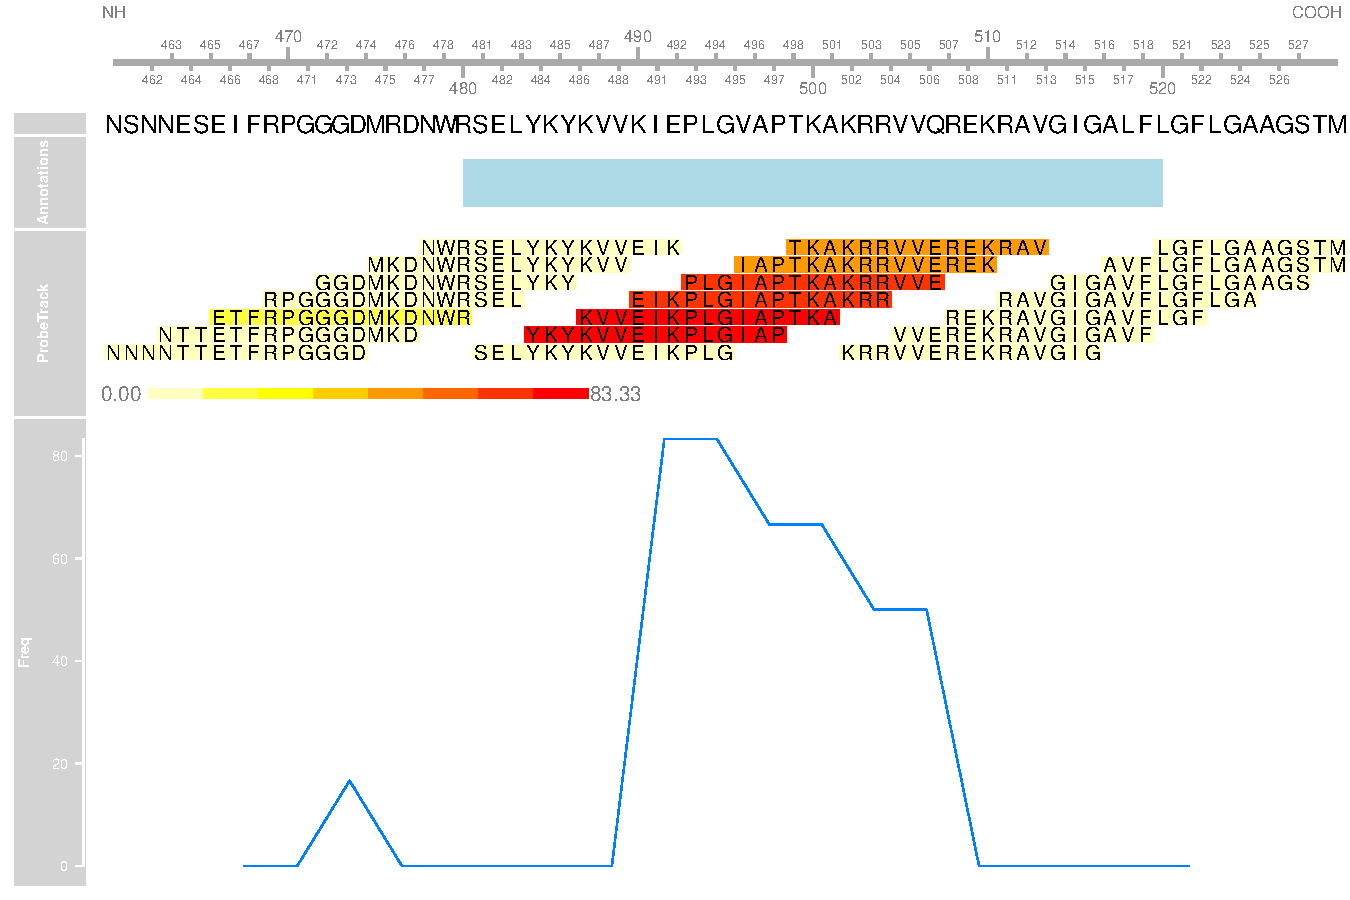
\includegraphics{Pviz-complex-plot}





\end{document}
